\chapter{Reduction, global operations}

In this exercise, we used the MPI function \textit{MPI\_Reduce} with the reduce operation \textit{MPI\_SUM}. The result of the program is shown by the following picture:
\begin{figure}[!h]
\begin{center}
	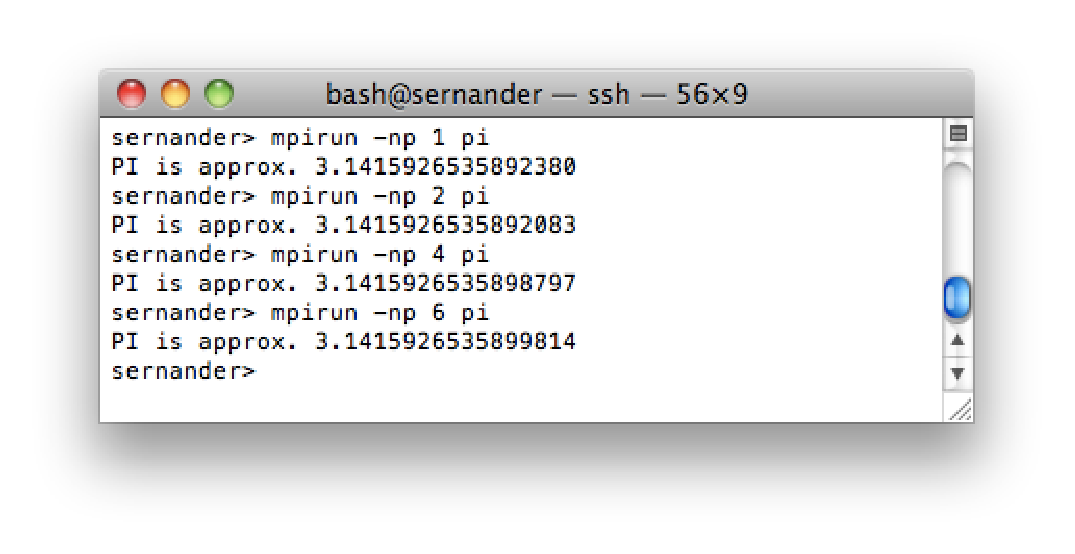
\includegraphics[width=\textwidth]{pic/pi.eps}
	\caption{Value of $\pi$ on a different number of processors}
\end{center}
\end{figure}

The results are a correct approximation of $\pi$, proof that the program does what it is designed for.

